%!TEX root = ../main.tex
\section{System Description}
\label{sec:system_description}
This project aims to develop an embedded system for monitoring parameters on the SDU go-kart.
\mikkel{Maybe some more text here?}
\subsection{SDU go-kart}
The SDU go-kart is an electronic go-kart equipped with a PMAC motor. 
To control the motor there is a sevcon gen4 motor controller mounted on the go-kart, but other inverters could be mounted and used instead.
It has a pedal for controlling the torque produced by the motor and a conventional disc brake with the break pedal connected using hydraulics.
It has four SB12V20P-FC \footnote{Super B 'Super-B - SB12V20P-FC LiFepo4 battery.pdf - reference datasheet'.} batteries put in series, yielding a combined nominal voltage of 52.8V and a discharge current of 560A.
The PMAC motor installed on the go-kart is a three phase motor capable of producing 6hp continuously.
The go-kart can be seen in figure \ref{fig:go_kart}.

\begin{figure}[h]
 	\centering
    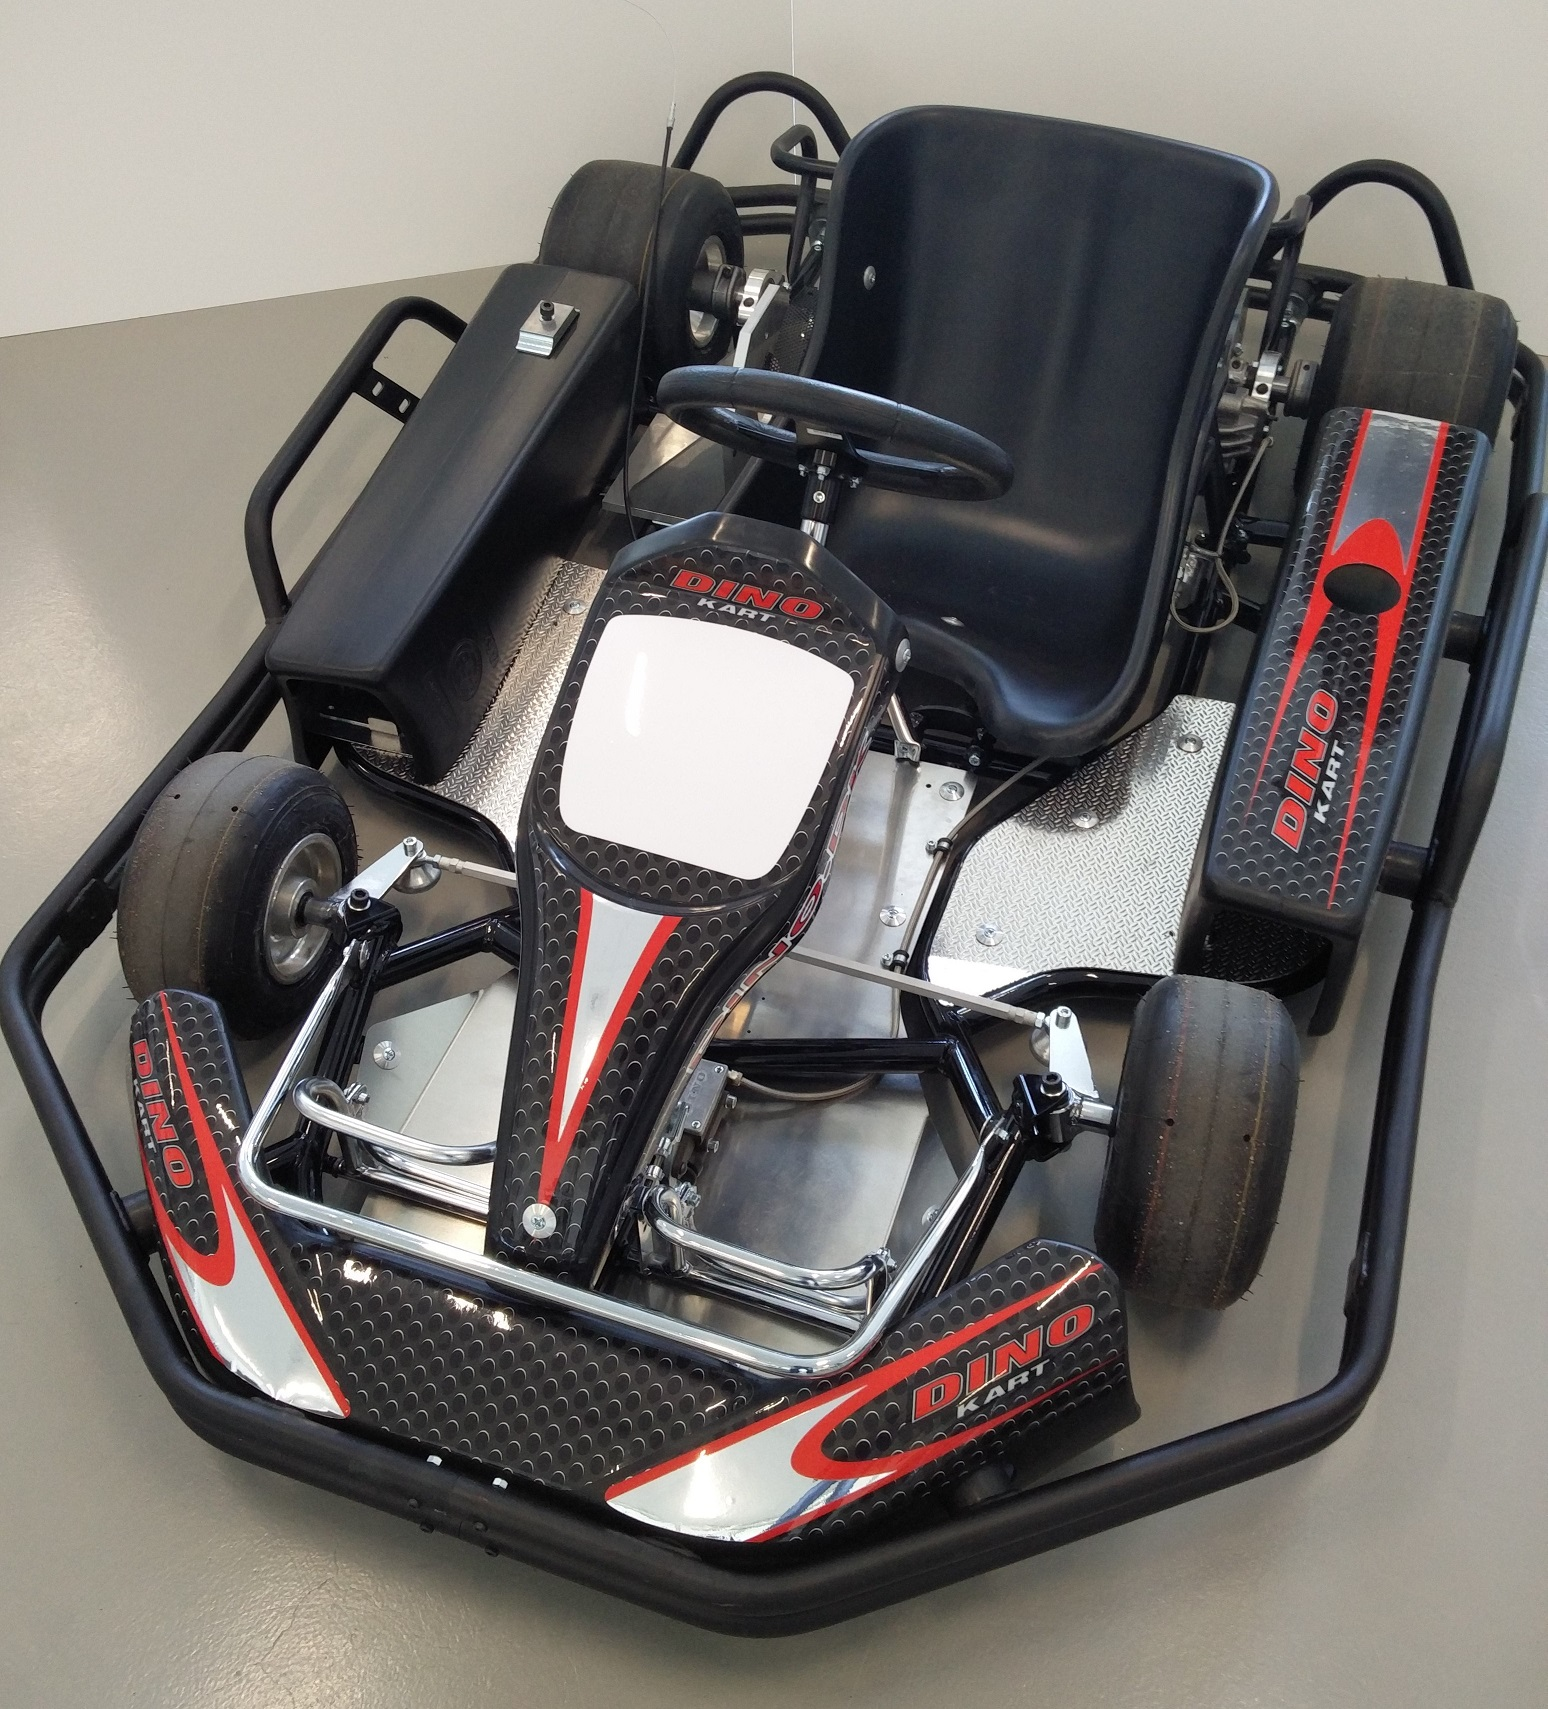
\includegraphics[width=0.4\textwidth]{graphics/go_kart}
    \caption{The SDU go-kart}
    \label{fig:go_kart}
\end{figure}

\catalin{We cannot state that each year the students will do this.}
The SDU go-kart is used as a development platform for students at the Master of Electronics educations at SDU.
Each year first semester students need to develop a three phase inverter to drive the go-kart.

\catalin{The two sentences with "there needs" might need rephrasing.}
\subsection{Embedded System}
To ease development on the go-kart lecturers and students would like to be able to monitor parameters on the go-kart while driving.
To collect data on the go-kart there needs to be sensors and microcontrollers on the go-kart.
To monitor while driving there needs to be a wireless connection between the go-kart and a stationary computer, see figure \ref{fig:simple}.
Data should be presented to the user on a UI on the stationary computer.
All data should also be logged locally on the go-kart, as there might be wireless network failures. 
It should be possible to start or stop data collecting for specific sensors.
\begin{figure}[h]
 	\centering
    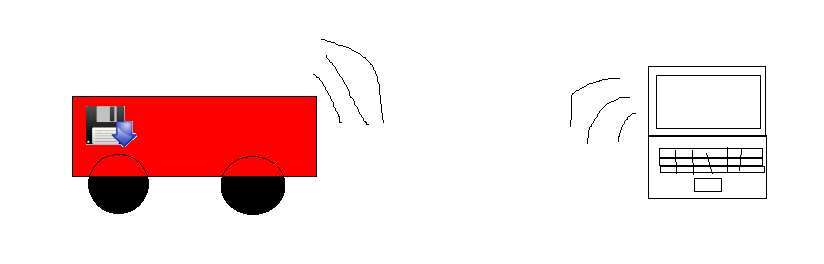
\includegraphics[width=0.6\textwidth]{graphics/go_kart_network_simple}
    \caption{SDU go-kart transferring data to a stationary computer wirelessly.}
    \label{fig:simple}
\end{figure}

A basic use case diagram showing the desired functionality of the embedded system can be seen in figure \ref{fig:use_cases}.
The use case narratives are shown in tables \ref{tab:use_monitor} to \ref{tab:use_start_stop}.


\begin{figure}[h]
 	\centering
    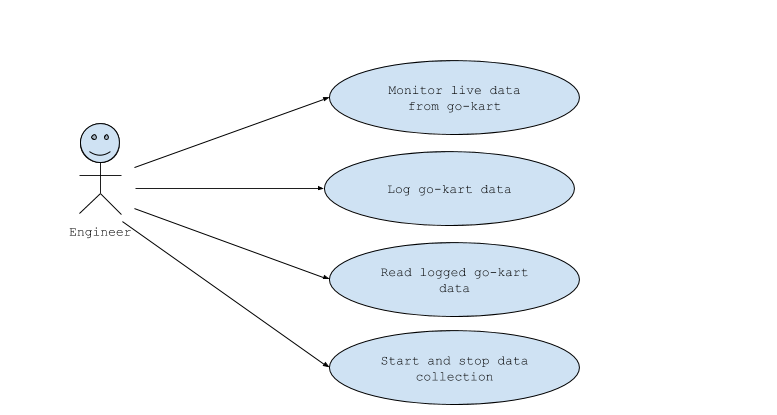
\includegraphics[width=1\textwidth]{graphics/use_cases.png}
    \caption{Use case diagram for the system.}
    \label{fig:use_cases}
\end{figure}

\begin{table}[H]
\centering
\caption{Usecase narrative for monitor live data from go-kart.}
\label{tab:use_monitor}
\begin{tabular}{| r | p{7 cm} |}
\hline
\textbf{Use case:}                        & Monitor live data from go-kart                  \\ 
\textbf{Actors:}                          & Engineer                                        \\
\textbf{Purpose:}                         & Monitor live data from go-kart while driving    \\
\textbf{Overview:}                        & The engineer starts the system. The system will begin collecting data on the go-kart and transfer them to a stationary computer. The computer will present data to the engineer on a UI. \\
\textbf{Type:}                            & Essential                                       \\
\textbf{Preconditions:}                   & Go-kart microcontroller is paired with stationary computer                                    \\
\textbf{Postconditions:}                  & System transfers data from go-kart sensors to a stationary computer, showing data in a UI.                                                                                            \\
\textbf{Special requirements:}            & -                                               \\ \hline 
\multicolumn{1}{|c|}{\textbf{Actor action}} & \multicolumn{1}{c|}{\textbf{System response}}\\
\multicolumn{1}{|p{5 cm}|}{1. Start system}       & \begin{tabular}[c]{@{}l@{}}2. Start collecting data\\ 3. Transfer data to stationary computer\\ 4. Present data in UI\end{tabular}                                              \\ \hline
\multicolumn{2}{|c|}{\textbf{Alternative flow of events}}                                   \\
\multicolumn{2}{|p{12 cm}|}{Any line: User can stop the system at any point in time.}              \\ \hline                                                                                                                                    
\end{tabular}
\end{table}


\begin{table}[H]
\centering
\caption{Usecase narrative for log go-kart data.}
\label{tab:use_log}
\begin{tabular}{| r | p{7 cm} |}
\hline
\textbf{Use case:}                        & Log go-kart data            			        \\ 
\textbf{Actors:}                          & Engineer                                        \\
\textbf{Purpose:}                         & Log go-kart data                 				\\
\textbf{Overview:}                        & After startup the system will log the collected data locally on the go-kart  \\
\textbf{Type:}                            & Essential                                       \\
\textbf{Preconditions:}                   & System is running and collecting go-kart data   \\
\textbf{Postconditions:}                  & System logs collected go-kart data.      		\\
\textbf{Special requirements:}            & -                                               \\ \hline 
\multicolumn{1}{|c|}{\textbf{Actor action}} & \multicolumn{1}{c|}{\textbf{System response}} \\
\multicolumn{1}{|p{5 cm}|}{}       & \begin{tabular}[c]{@{}l@{}}1. Log collected data locally on go-kart\end{tabular}\\ \hline
\multicolumn{2}{|c|}{\textbf{Alternative flow of events}}                                   \\
\multicolumn{2}{|p{12 cm}|}{Any line: User can stop the logging	at any point in time.}         \\ \hline                                                                                                                                    
\end{tabular}
\end{table}



\begin{table}[H]
\centering
\caption{Usecase narrative for read logged data.}
\label{tab:use_read_log}
\begin{tabular}{| r | p{7 cm} |}
\hline
\textbf{Use case:}                        & Read logged data  			                    \\ 
\textbf{Actors:}                          & Engineer                                        \\
\textbf{Purpose:}                         & To read data that is logged locally on the go-kart               \\
\textbf{Overview:}                        & The engineer will ask the system for the logged data. The system will transfer the logged data to a stationary computer \\
\textbf{Type:}                            & Essential                                       \\
\textbf{Preconditions:}                   & Data is logged in logfile on the go-kart                \\
\textbf{Postconditions:}                  & The log file is on the stationary computer                                                                                      \\
\textbf{Special requirements:}            & -                                               \\ \hline 
\multicolumn{1}{|c|}{\textbf{Actor action}} & \multicolumn{1}{c|}{\textbf{System response}}\\
\multicolumn{1}{|p{5 cm}|}{1. Ask for log file}       & \begin{tabular}[c]{@{}l@{}}2. Transfer logged data to stationary computer\\ 3. Save data to log file on stationary computer\end{tabular}                                              \\ \hline
\multicolumn{2}{|c|}{\textbf{Alternative flow of events}}                                   \\
\multicolumn{2}{|p{12 cm}|}{Any line: If connection is lost the system should detect it and mark the trasferred log file as invalid}              \\ \hline                                                                                                                                    
\end{tabular}
\end{table}

\begin{table}[H]
\centering
\caption{Usecase narrative for start and stop data collection.}
\label{tab:use_start_stop}
\begin{tabular}{| r | p{7 cm} |}
\hline
\textbf{Use case:}                        & Start and stop data collection  			                    \\ 
\textbf{Actors:}                          & Engineer                                        \\
\textbf{Purpose:}                         & To start and stop data collection from specified sensors              \\
\textbf{Overview:}                        & The engineer will ask the system to start or stop collecting data from a specific sensor. The system will then start or stop the system respectively. \\
\textbf{Type:}                            & Important                                       \\
\textbf{Preconditions:}                   & System is running               \\
\textbf{Postconditions:}                  & Data collecting is started or stopped for specific sensor.                                                                                      \\
\textbf{Special requirements:}            & -                                               \\ \hline 
\multicolumn{1}{|c|}{\textbf{Actor action}} & \multicolumn{1}{c|}{\textbf{System response}}\\
\multicolumn{1}{|p{5 cm} |}{1. Ask system to start or stop data collecting for specific sensor.}       & \begin{tabular}[c]{@{}p{7cm}@{}}2. System starts or stops data collecting for specific sensor\end{tabular}                              	                \\ \hline
\multicolumn{2}{|c|}{\textbf{Alternative flow of events}}                                   \\
\multicolumn{2}{|p{12 cm}|}{-}              \\ \hline                                                                                                                                    
\end{tabular}
\end{table}


%Relavant control variables should be controllable, while driving allowing for efficient testing of controllers.
%To achieve this, data should be collected on a computer on the go-kart and sent to a stationary computer.

%\subsection{What is the role of transferring go-kart data to and from a stationary computer?}
%To let an engineer or a mechanic monitor the status of the go-kart.

%Movement data could be usefull for testing new hardware, improving existing hardware and evaluation the drivers performance. 
%Data about battery status, currents, motortemperature is usefull for safety procedures.
%Data from the SEVCON xxx inverter or other inverters on the go-kart could be used for tuning parameters, evaluation performance and safety measures.
%On the basis of this data it should be possibly to change configuration parameters on the SEVCON xxx while driving the go-kart.

%\subsection{What is the role of the stationary computer?}
%The stationary computer should be responsible of the transmission of relevant go-kart data to and from the "on-board" computer.
%The received data should be presented to the user in a SCADA system.

%\subsubsection*{What data and sensors would be interesting to monitor?}
%Data from IMU, GPS and encoders would be necessary to monitor the movement of the go-kart.
%Data from the SEVCON xxx gives information about about battery status, currents, motortemperature.
%Temperature of tyres, speed of front wheels, possibility to control or at least moniter stearing and brake.
%It should be possible to get data from a new inverter, that is not yet made. 

%\subsubsection*{What kind is the stationary computer?}
%It should be possible for different personnel to monitor the go-kart data therefore the statinonary computer should just be general purpose computer running (linux?).

%\subsubsection*{What kind of communication is needed to transfer data between the go-kart computer and the stationary computer?}
%As it should be possibly to monitor data while the go-kart is driving the connection clearly needs to be wireless with a range allowing for driving on a typical racing track. 
%As all data is used by humans the propagation delay of the connection is not required to be very low.


%As live data should be easy to read? ("overskue" in danish) there needs to be a GUI or at least a UI that will present the user with easy readable data. SCADA SYSTEM!?!?!
%Changing of parameters on the go-kart should also be in the UI in order useable by others than the developers.

%\subsection{What is the role of the computer on the go-kart?}
%The "onboard" computer needs to handle the collection
%of data from different sensors (data producers).
%This computer will also handle the transmission of data to the stationary 
%computer.
%There are tasks that need to be handled locally fx strict safety measures (and future things fx localisation) that requires a miminum delay. 
%Storing of data with a 
%The computer needs also to store data locally in order to avoid data loss if the wireless connection is lost.

%\subsubsection*{How is local data transmission handled?}
%All data should be collected locally on the "on-board" computer to transmit it to the stationary computer.
%Local data collection should be "fast" and "reliable" for local safety measures to function properly.
%It should be possibly to collect data from and transmit data to at least the 
%aforementioned IMU, GPS and SEVCON xx with the possibility of adding additional 
%data producers.

%\subsubsection*{What kind is the "on-board" computer?}
%The computer should be a small embedded platform in order to mount it physcically on the go-kart.
%It should be able to handle all "on-board" tasks.

%Data should be stored directly on nonvolatile memory to be able retrieve data after shutdown.
%Data integrity checks is needed to ensure proper data logging.
%Correct data logging should be realised to ensure validity of data. 


